\documentclass[tikz,border=5pt]{standalone}
\usepackage[T1]{fontenc}
\usepackage{lmodern,amsmath,amssymb}
\usetikzlibrary{arrows.meta,calc,positioning,fit,backgrounds,shapes.geometric,matrix,decorations.pathreplacing,patterns}
\definecolor{ink}{gray}{0.08}
\definecolor{wash}{gray}{0.965}
\definecolor{soft}{gray}{0.45}
\tikzset{box/.style={draw=ink,line width=.65pt,fill=white,align=center,inner sep=4pt,outer sep=0pt,font=\small},flow/.style={draw=ink,line width=.65pt,-{Latex[length=1.8mm,width=1.3mm]},rounded corners=2pt},annotation/.style={font=\scriptsize,text=soft,align=center},groupbox/.style={draw=soft,dashed,line width=.45pt,fill=wash}}
\begin{document}
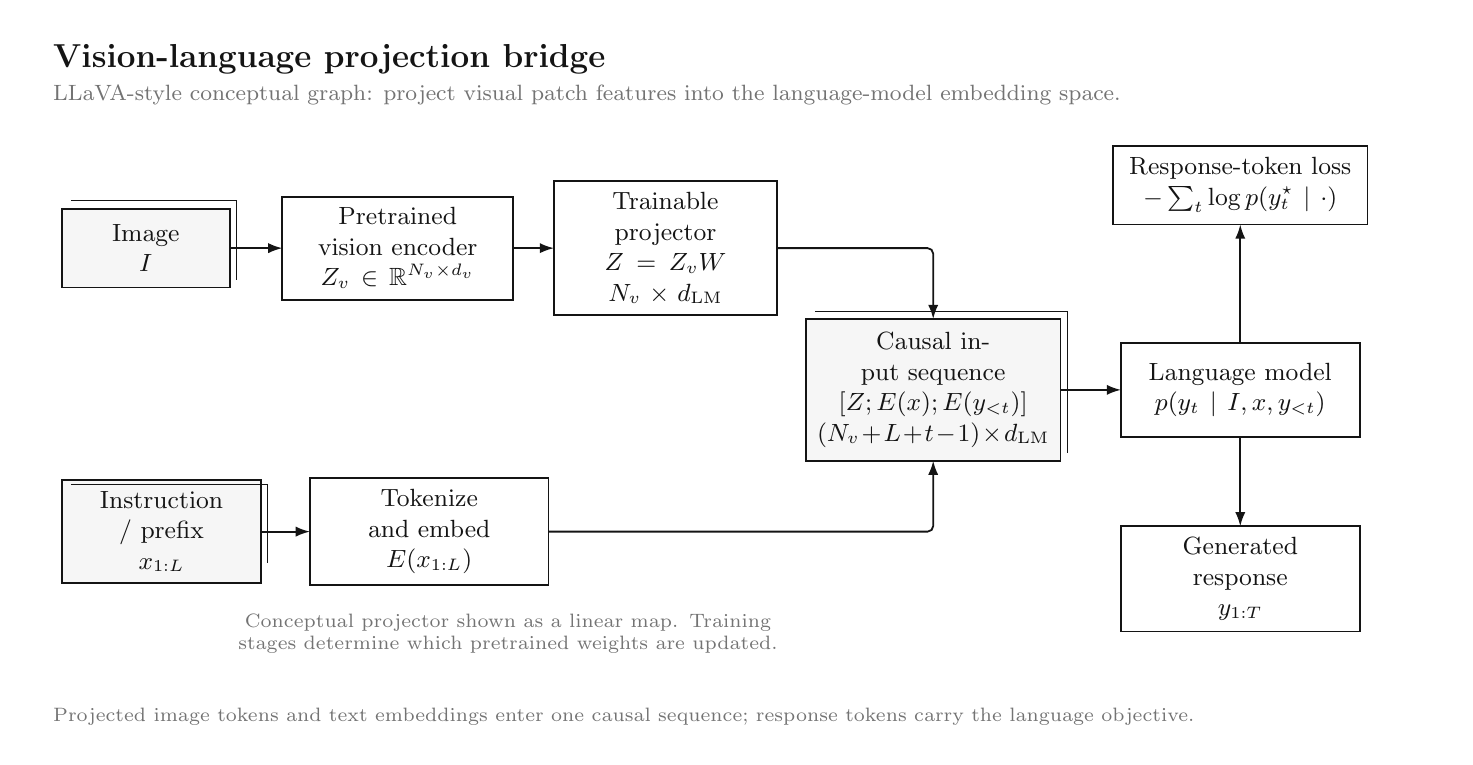
\begin{tikzpicture}[x=1cm,y=-1cm,font=\rmfamily,text=ink]

\path[use as bounding box] (0,0) rectangle (18,9);
\node[anchor=west,font=\large\bfseries] at (.2,.4) {Vision-language projection bridge};
\node[anchor=west,font=\footnotesize,text=soft] at (.2,.85) {LLaVA-style conceptual graph: project visual patch features into the language-model embedding space.};
\begin{pgfonlayer}{background}
\end{pgfonlayer}
\node[box,fill=wash,minimum width=2.1cm,minimum height=1cm,text width=1.85cm] (image) at (1.5,2.8) {Image\\$I$};
\draw[ink,line width=.4pt] (0.5499999999999999,2.1999999999999997) -- (2.65,2.1999999999999997) -- (2.65,3.1999999999999997);
\node[box,minimum width=2.9cm,minimum height=1.2cm,text width=2.65cm] (vision) at (4.7,2.8) {Pretrained vision encoder\\$Z_v\in\mathbb{R}^{N_v\times d_v}$};
\node[box,minimum width=2.8cm,minimum height=1.4cm,text width=2.55cm] (proj) at (8.1,2.8) {Trainable projector\\$Z=Z_vW$\\$N_v\times d_{\mathrm{LM}}$};
\node[box,fill=wash,minimum width=2.5cm,minimum height=1cm,text width=2.25cm] (instruction) at (1.7,6.4) {Instruction / prefix\\$x_{1:L}$};
\draw[ink,line width=.4pt] (0.5499999999999999,5.800000000000001) -- (3.0500000000000003,5.800000000000001) -- (3.0500000000000003,6.800000000000001);
\node[box,minimum width=3.0cm,minimum height=1.1cm,text width=2.75cm] (tokenize) at (5.1,6.4) {Tokenize and embed\\$E(x_{1:L})$};
\node[box,fill=wash,minimum width=3.2cm,minimum height=1.8cm,text width=2.95cm] (sequence) at (11.5,4.6) {Causal input sequence\\$[Z;E(x);E(y_{<t})]$\\$(N_v+L+t-1)\times d_{\mathrm{LM}}$};
\draw[ink,line width=.4pt] (10.0,3.5999999999999996) -- (13.2,3.5999999999999996) -- (13.2,5.4);
\node[box,minimum width=3.0cm,minimum height=1.2cm,text width=2.75cm] (lm) at (15.4,4.6) {Language model\\$p(y_t\mid I,x,y_{<t})$};
\node[box,minimum width=3.2cm,minimum height=1.0cm,text width=2.95cm] (loss) at (15.4,2.0) {Response-token loss\\$-\sum_t\log p(y_t^{\star}\mid\cdot)$};
\node[box,minimum width=3.0cm,minimum height=0.9cm,text width=2.75cm] (response) at (15.4,7.0) {Generated response\\$y_{1:T}$};
\begin{pgfonlayer}{background}
\draw[flow] (image.east) -- (vision.west);
\draw[flow] (vision.east) -- (proj.west);
\draw[flow] (instruction.east) -- (tokenize.west);
\draw[flow] (proj.east) -- (11.5,2.8) -- (sequence.north);
\draw[flow] (tokenize.east) -- (11.5,6.4) -- (sequence.south);
\draw[flow] (sequence.east) -- (lm.west);
\draw[flow] (lm.north) -- (loss.south);
\draw[flow] (lm.south) -- (response.north);
\end{pgfonlayer}
\node[annotation,text width=9.8cm] at (6.1,7.7) {Conceptual projector shown as a linear map. Training stages determine which pretrained weights are updated.};
\node[anchor=west,align=left,font=\scriptsize,text=soft,text width=17.6cm] at (.2,8.75) {Projected image tokens and text embeddings enter one causal sequence; response tokens carry the language objective.};
\end{tikzpicture}
\end{document}
